\setcounter{secnumdepth}{3}
\titlespacing*{\chapter}{0pt}{-0.1cm}{1cm}
\titleformat{\chapter}[display]
  {\bfseries\LARGE}  
  {Phần~\thechapter}{0pt}{\raggedright}

\chapter{Kết quả thực nghiệm}
Để đảm bảo hiệu năng, quá trình chạy benchmark được trang bị cơ chế \textit{timeout}, tự động dừng quá trình tìm kiếm nếu vượt quá thời gian cho phép, từ đó tránh việc tiêu tốn tài nguyên không cần thiết.
\section{Input-01}
\textbf{Mô tả testcase:}
Testcase Futoshiki kích thước $3 \times 3$ với độ khó thấp. Số lượng ô được điền ban đầu (clues) rất ít (chỉ 1 ô), tạo ra không gian tìm kiếm vừa phải.

Các ràng buộc (constraints) tồn tại nhưng mật độ thấp: chỉ 1 ràng buộc ngang và 2 ràng buộc dọc, phân bố không đồng đều. Bài toán có tính chất đơn giản và các phương pháp tìm kiếm dễ dàng tìm được nghiệm.

Đây là testcase cơ bản để kiểm tra khả năng hoạt động của các thuật toán trên bài toán nhỏ và không phức tạp.

\begin{center}
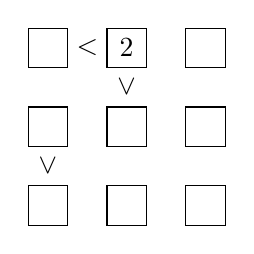
\begin{tikzpicture}[scale=0.5]

% ===== Vẽ các ô (rời nhau) =====
\foreach \x in {0,2,4} {
    \foreach \y in {0,2,4} {
        \draw (\x,\y) rectangle ++(1,1);
    }
}

% ===== Điền số =====
\node at (2.5,4.5) {2};

% ===== Horizontal constraints =====
\node at (0.5+1,4.5) {$<$};

% ===== Vertical constraints =====
\node at (2.5,3.5) {$\vee$};
\node at (0.5,1.5) {$\vee$};

\end{tikzpicture}
\end{center}

\textbf{Kết quả:}
\begin{table}[H]
\centering
\begin{tabular}{|l|l|c|c|c|c|c|}
\hline
\textbf{Input} & \textbf{Method} & \textbf{Runtime (s)} & \textbf{Memory (MB)} & \textbf{Nodes} & \textbf{Solved} & \textbf{Timeout} \\
\hline
input\_01.txt & Forward Chaining & 0.01 & 0.11 & 1 & True & False \\
input\_01.txt & A* (Heuristic 1) & 0.002 & 0.02 & 11 & True & False \\
input\_01.txt & A* (Heuristic 2) & 0.005 & 0.02 & 9 & True & False \\
input\_01.txt & Brute Force & 0.0004 & 0.01 & 16 & True & False \\
input\_01.txt & Backtracking & 0.0001 & 0.0 & 11 & True & False \\
\hline
\end{tabular}
\caption{Kết quả benchmark cho input\_01.txt}
\end{table}

\paragraph{So sánh và đánh giá:}

\begin{itemize}
\item \textbf{Forward Chaining:}
\begin{itemize}
    \item Thời gian chạy ngắn (0.006s), bộ nhớ sử dụng thấp (0.11MB), mở rộng chỉ 1 node.
    \item Tìm được nghiệm thành công.
    \item Phương pháp suy luận tiến hiệu quả do constraint propagation nhanh chóng xác định các giá trị từ các ràng buộc ít ỏi.
\end{itemize}

\item \textbf{A* với Heuristic 1:}
\begin{itemize}
    \item Thời gian chạy rất ngắn (0.002s), bộ nhớ rất thấp (0.02MB), mở rộng 11 nodes.
    \item Tìm được nghiệm thành công.
    \item A* với Heuristic 1 tuy tốt hơn Forward Chaining về thời gian nhưng mở rộng nhiều node hơn, cho thấy heuristic 1 không hoàn toàn chính xác.
\end{itemize}

\item \textbf{A* với Heuristic 2:}
\begin{itemize}
    \item Thời gian chạy ngắn (0.005s), bộ nhớ thấp (0.02MB), mở rộng 9 nodes.
    \item Tìm được nghiệm thành công.
    \item Heuristic 2 cải thiện đáng kể, mở rộng ít node hơn Heuristic 1 (9 vs 11), cho thấy heuristic 2 dẫn dắt tìm kiếm hiệu quả hơn.
\end{itemize}

\item \textbf{Brute Force:}
\begin{itemize}
    \item Thời gian chạy rất ngắn (0.0004s), mở rộng 16 nodes.
    \item Tìm được nghiệm thành công.
    \item Do không gian tìm kiếm nhỏ (3x3), brute force vẫn chạy nhanh mặc dù không có cắt tỉa.
\end{itemize}

\item \textbf{Backtracking:}
\begin{itemize}
    \item Thời gian chạy cực nhanh (0.0001s), mở rộng 11 nodes, bộ nhớ tối thiểu (0.0MB).
    \item Tìm được nghiệm thành công.
    \item Backtracking là phương pháp nhanh nhất cho testcase nhỏ này nhờ cắt tỉa hiệu quả và chi phí thấp.
\end{itemize}

\end{itemize}

\textbf{So sánh tổng thể:}

\begin{itemize}
    \item Về \textbf{tốc độ}:
    \begin{itemize}
        \item Backtracking nhanh nhất (0.0001s), tiếp theo là A* Heuristic 1 (0.002s).
        \item Forward Chaining chậm hơn do chi phí suy luận ràng buộc.
    \end{itemize}
    
    \item Về \textbf{hiệu quả heuristic}:
    \begin{itemize}
        \item Heuristic 2 tốt hơn Heuristic 1 (mở rộng 9 vs 11 nodes).
        \item Cả hai heuristic đều hiệu quả cho bài toán nhỏ này.
    \end{itemize}
    
    \item Về \textbf{khả năng tìm kiếm}:
    \begin{itemize}
        \item Tất cả phương pháp đều tìm được nghiệm thành công.
        \item Sự khác biệt về performance là nhỏ do kích thước bài toán đơn giản.
    \end{itemize}
\end{itemize}


\section{Input-02}
\textbf{Mô tả testcase:}
Testcase Futoshiki kích thước $4 \times 4$ với độ khó dễ. Số lượng ô được điền ban đầu (clues) rất ít (chỉ 1 ô), tạo ra không gian tìm kiếm tương đối nhỏ.

Các ràng buộc (constraints) phân bố vừa phải: 3 ràng buộc ngang và 2 ràng buộc dọc. Bài toán có tính chất quản lý được và các phương pháp tìm kiếm với cắt tỉa hoạt động tốt.

Đây là testcase trung gian giữa các bài toán nhỏ và bài toán phức tạp hơn, phù hợp để đánh giá khả năng mở rộng của các thuật toán.

\begin{center}
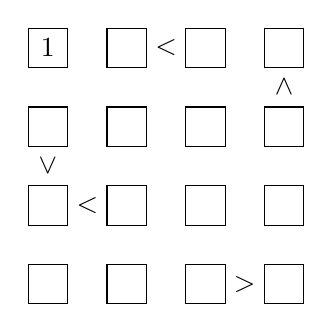
\begin{tikzpicture}[scale=0.5]

% ===== Vẽ các ô (rời nhau) =====
\foreach \x in {0,2,4,6} {
    \foreach \y in {0,2,4,6} {
        \draw (\x,\y) rectangle ++(1,1);
    }
}

% ===== Điền số =====
\node at (0.5,6.5) {1};

% ===== Horizontal constraints =====
\node at (2.5+1,6.5) {$<$};

\node at (0.5+1,2.5) {$<$};

\node at (4.5+1,0.5) {$>$};

% ===== Vertical constraints =====
\node at (6.5,5.5) {$\wedge$};

\node at (0.5,3.5) {$\vee$};

\end{tikzpicture}
\end{center}

\textbf{Kết quả:}
\begin{table}[H]
\centering
\begin{tabular}{|l|l|c|c|c|c|c|}
\hline
\textbf{Input} & \textbf{Method} & \textbf{Runtime (s)} & \textbf{Memory (MB)} & \textbf{Nodes} & \textbf{Solved} & \textbf{Timeout} \\
\hline
input\_02.txt & Forward Chaining & 0.08 & 1.34 & 21 & True & False \\
input\_02.txt & A* (Heuristic 1) & 0.05 & 0.3 & 135 & True & False \\
input\_02.txt & A* (Heuristic 2) & 0.02 & 0.07 & 16 & True & False \\
input\_02.txt & Brute Force & 0.08 & 1.95 & 803 & True & False \\
input\_02.txt & Backtracking & 0.002 & 0.19 & 84 & True & False \\
\hline
\end{tabular}
\caption{Kết quả benchmark cho input\_02.txt}
\end{table}

\paragraph{So sánh và đánh giá:}

\begin{itemize}
\item \textbf{Forward Chaining:}
\begin{itemize}
    \item Thời gian chạy 0.08s, bộ nhớ 1.34MB, mở rộng 21 nodes.
    \item Tìm được nghiệm thành công.
    \item Chi phí suy luận ràng buộc tăng lên khi kích thước bài toán lớn hơn, nhưng vẫn quản lý được.
\end{itemize}

\item \textbf{A* với Heuristic 1:}
\begin{itemize}
    \item Thời gian chạy 0.05s, bộ nhớ 0.3MB, mở rộng 135 nodes.
    \item Tìm được nghiệm thành công.
    \item Hiệu quả hơn Forward Chaining về thời gian nhưng mở rộng nhiều node hơn, cho thấy heuristic 1 chưa đủ mạnh cho bài toán này.
\end{itemize}

\item \textbf{A* với Heuristic 2:}
\begin{itemize}
    \item Thời gian chạy 0.02s, bộ nhớ 0.07MB, mở rộng 16 nodes.
    \item Tìm được nghiệm thành công.
    \item Heuristic 2 vượt trội với thời gian nhanh nhất và mở rộng ít node nhất, cho thấy tính hiệu quả cao của heuristic này.
\end{itemize}

\item \textbf{Brute Force:}
\begin{itemize}
    \item Thời gian chạy 0.08s, bộ nhớ cao (1.95MB), mở rộng 803 nodes.
    \item Tìm được nghiệm thành công.
    \item Mở rộng gấp 50 lần so với A* Heuristic 2 (803 vs 16), cho thấy nhược điểm của phương pháp không cắt tỉa.
\end{itemize}

\item \textbf{Backtracking:}
\begin{itemize}
    \item Thời gian chạy rất ngắn (0.002s), bộ nhớ 0.19MB, mở rộng 84 nodes.
    \item Tìm được nghiệm thành công.
    \item Backtracking là phương pháp nhanh thứ hai sau A* Heuristic 2, nhưng hiệu quả tìm kiếm thấp hơn do mở rộng nhiều node hơn.
\end{itemize}

\end{itemize}

\textbf{So sánh tổng thể:}

\begin{itemize}
    \item Về \textbf{tốc độ}:
    \begin{itemize}
        \item Backtracking nhanh nhất (0.002s), A* Heuristic 2 thứ hai (0.02s).
        \item Brute Force và Forward Chaining chậm hơn đáng kể (0.08s).
    \end{itemize}
    
    \item Về \textbf{hiệu quả heuristic}:
    \begin{itemize}
        \item Heuristic 2 là tối ưu, mở rộng chỉ 16 nodes (ít nhất).
        \item Heuristic 1 kém hơn, mở rộng 135 nodes (gần 8 lần nhiều hơn).
    \end{itemize}
    
    \item Về \textbf{chi phí bộ nhớ}:
    \begin{itemize}
        \item A* Heuristic 2 tiết kiệm bộ nhớ nhất (0.07MB).
        \item Brute Force tiêu tốn nhiều bộ nhớ nhất (1.95MB).
    \end{itemize}
\end{itemize}


\section{Input-03}
\textbf{Mô tả testcase:}
Testcase Futoshiki kích thước $5 \times 5$ với độ khó trung bình. Số lượng ô được điền ban đầu (clues) vẫn rất ít (chỉ 1 ô), nhưng không gian tìm kiếm bắt đầu tăng đáng kể.

Các ràng buộc (constraints) phân bố đều hơn: 5 ràng buộc ngang và 3 ràng buộc dọc, giúp cắt tỉa không gian tìm kiếm. Bài toán bắt đầu cho thấy sự khác biệt rõ rệt giữa các phương pháp tìm kiếm, đặc biệt là tác dụng của cắt tỉa và heuristic.

Đây là điểm tới hạn nơi các thuật toán yếu kém bắt đầu gặp khó khăn.

\begin{center}
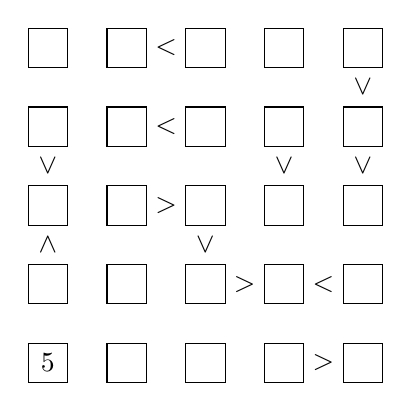
\begin{tikzpicture}[scale=0.5]

% ===== Vẽ các ô (rời nhau) =====
\foreach \x in {0,2,4,6,8} {
    \foreach \y in {0,2,4,6,8} {
        \draw (\x,\y) rectangle ++(1,1);
    }
}

% ===== Điền số =====
\node at (0.5,0.5) {5};

% ===== Horizontal constraints =====
\node at (2.5+1,8.5) {$<$};

\node at (2.5+1,6.5) {$<$};

\node at (2.5+1,4.5) {$>$};

\node at (4.5+1,2.5) {$>$};
\node at (6.5+1,2.5) {$<$};

\node at (6.5+1,0.5) {$>$};

% ===== Vertical constraints =====
\node at (8.5,7.5) {$\vee$};

\node at (0.5,5.5) {$\vee$};
\node at (6.5,5.5) {$\vee$};
\node at (8.5,5.5) {$\vee$};

\node at (0.5,3.5) {$\wedge$};
\node at (4.5,3.5) {$\vee$};

\end{tikzpicture}
\end{center}

\textbf{Kết quả:}
\begin{table}[H]
\centering
\begin{tabular}{|l|l|c|c|c|c|c|}
\hline
\textbf{Input} & \textbf{Method} & \textbf{Runtime (s)} & \textbf{Memory (MB)} & \textbf{Nodes} & \textbf{Solved} & \textbf{Timeout} \\
\hline
input\_03.txt & Forward Chaining & 1.23 & 6.06 & 156 & True & False \\
input\_03.txt & A* (Heuristic 1) & 2.55 & 15.74 & 4,466 & True & False \\
input\_03.txt & A* (Heuristic 2) & 0.15 & 0.35 & 37 & True & False \\
input\_03.txt & Brute Force & 3.58 & 0.14 & 56,318 & True & False \\
input\_03.txt & Backtracking & 0.05 & 4.73 & 1,459 & True & False \\
\hline
\end{tabular}
\caption{Kết quả benchmark cho input\_03.txt}
\end{table}

\paragraph{So sánh và đánh giá:}

\begin{itemize}
\item \textbf{Forward Chaining:}
\begin{itemize}
    \item Thời gian chạy 1.23s, bộ nhớ 6.06MB, mở rộng 156 nodes.
    \item Tìm được nghiệm thành công.
    \item Chi phí suy luận tăng lên khi bài toán phức tạp hơn, nhưng vẫn tìm được nghiệm hiệu quả hơn so với một số phương pháp tìm kiếm ngây thơ.
\end{itemize}

\item \textbf{A* với Heuristic 1:}
\begin{itemize}
    \item Thời gian chạy chậm nhất (2.55s), bộ nhớ cao nhất (15.74MB), mở rộng 4,466 nodes.
    \item Tìm được nghiệm thành công.
    \item Heuristic 1 cho kết quả tồi tệ trên bài toán này, mở rộng gấp 120 lần so với Heuristic 2 (4,466 vs 37), cho thấy heuristic 1 không phù hợp cho bài toán lớn hơn.
\end{itemize}

\item \textbf{A* với Heuristic 2:}
\begin{itemize}
    \item Thời gian chạy 0.15s, bộ nhớ tối thiểu (0.35MB), mở rộng 37 nodes.
    \item Tìm được nghiệm thành công.
    \item A* Heuristic 2 là phương pháp tốt nhất cho testcase này, nhanh gấp 8 lần so với Forward Chaining và gấp 17 lần so với Brute Force.
\end{itemize}

\item \textbf{Brute Force:}
\begin{itemize}
    \item Thời gian chạy 3.58s, bộ nhớ thấp (0.14MB), mở rộng 56,318 nodes.
    \item Tìm được nghiệm thành công.
    \item Mở rộng gần 1,500 lần so với A* Heuristic 2, cho thấy thiếu cắt tỉa và heuristic là rất tốn kém.
\end{itemize}

\item \textbf{Backtracking:}
\begin{itemize}
    \item Thời gian chạy 0.05s, bộ nhớ 4.73MB, mở rộng 1,459 nodes.
    \item Tìm được nghiệm thành công.
    \item Backtracking nhanh hơn Forward Chaining gấp 25 lần, nhưng vẫn chậm hơn A* Heuristic 2 gấp 3 lần do mở rộng nhiều node hơn.
\end{itemize}

\end{itemize}

\textbf{So sánh tổng thể:}

\begin{itemize}
    \item Về \textbf{tốc độ}:
    \begin{itemize}
        \item Backtracking nhanh nhất (0.05s), A* Heuristic 2 thứ hai (0.15s).
        \item Brute Force (3.58s) và A* Heuristic 1 (2.55s) chậm hơn nhiều.
    \end{itemize}
    
    \item Về \textbf{hiệu quả heuristic}:
    \begin{itemize}
        \item Heuristic 2 vượt trội hơn hết (37 nodes).
        \item Heuristic 1 gặp khó khăn lớn khi bài toán phức tạp (4,466 nodes).
    \end{itemize}
    
    \item Về \textbf{khả năng mở rộng}:
    \begin{itemize}
        \item A* Heuristic 2 cho thấy khả năng mở rộng tốt.
        \item Brute Force và Forward Chaining không mở rộng tốt khi kích thước bài toán tăng.
    \end{itemize}
\end{itemize}


\section{Input-04}
\textbf{Mô tả testcase:}
Testcase Futoshiki kích thước $5 \times 5$ với độ khó trung bình. Số lượng ô được điền ban đầu (clues) là 2 ô, nhiều hơn testcase trước, giúp giảm không gian tìm kiếm một chút.

Các ràng buộc (constraints) phân bố vừa phải: 4 ràng buộc ngang và 3 ràng buộc dọc. So với Input-03, Input-04 có thêm clue nhưng số constraints tương tự, dẫn đến bài toán dễ hơn một chút.

Testcase này cho thấy tác dụng của việc có nhiều clue hơn trong việc hạn chế không gian tìm kiếm.

\begin{center}
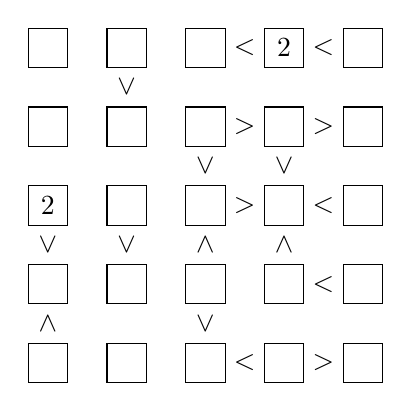
\begin{tikzpicture}[scale=0.5]

% ===== Vẽ các ô (rời nhau) =====
\foreach \x in {0,2,4,6,8} {
    \foreach \y in {0,2,4,6,8} {
        \draw (\x,\y) rectangle ++(1,1);
    }
}

% ===== Điền số =====
\node at (6.5,8.5) {2};
\node at (0.5,4.5) {2};

% ===== Horizontal constraints =====
\node at (4.5+1,8.5) {$<$};
\node at (6.5+1,8.5) {$<$};

\node at (4.5+1,6.5) {$>$};
\node at (6.5+1,6.5) {$>$};

\node at (4.5+1,4.5) {$>$};
\node at (6.5+1,4.5) {$<$};

\node at (6.5+1,2.5) {$<$};

\node at (4.5+1,0.5) {$<$};
\node at (6.5+1,0.5) {$>$};

% ===== Vertical constraints =====
\node at (2.5,7.5) {$\vee$};

\node at (4.5,5.5) {$\vee$};
\node at (6.5,5.5) {$\vee$};

\node at (0.5,3.5) {$\vee$};
\node at (2.5,3.5) {$\vee$};
\node at (4.5,3.5) {$\wedge$};
\node at (6.5,3.5) {$\wedge$};

\node at (0.5,1.5) {$\wedge$};
\node at (4.5,1.5) {$\vee$};

\end{tikzpicture}
\end{center}

\textbf{Kết quả:}
\begin{table}[H]
\centering
\begin{tabular}{|l|l|c|c|c|c|c|}
\hline
\textbf{Input} & \textbf{Method} & \textbf{Runtime (s)} & \textbf{Memory (MB)} & \textbf{Nodes} & \textbf{Solved} & \textbf{Timeout} \\
\hline
input\_04.txt & Forward Chaining & 1.21 & 5.35 & 120 & True & False \\
input\_04.txt & A* (Heuristic 1) & 0.41 & 2.5 & 746 & True & False \\
input\_04.txt & A* (Heuristic 2) & 0.10 & 0.28 & 29 & True & False \\
input\_04.txt & Brute Force & 7.03 & 0.15 & 109,458 & True & False \\
input\_04.txt & Backtracking & 0.02 & 2.37 & 750 & True & False \\
\hline
\end{tabular}
\caption{Kết quả benchmark cho input\_04.txt}
\end{table}

\paragraph{So sánh và đánh giá:}

\begin{itemize}
\item \textbf{Forward Chaining:}
\begin{itemize}
    \item Thời gian chạy 1.21s, bộ nhớ 5.35MB, mở rộng 120 nodes.
    \item Tìm được nghiệm thành công.
    \item Chi phí suy luận ổn định, mở rộng ít hơn Input-03 (120 vs 156) do có thêm clue giúp constraint propagation hiệu quả hơn.
\end{itemize}

\item \textbf{A* với Heuristic 1:}
\begin{itemize}
    \item Thời gian chạy 0.41s, bộ nhớ 2.5MB, mở rộng 746 nodes.
    \item Tìm được nghiệm thành công.
    \item Hiệu suất tốt hơn trên Input-04 so với Input-03 (0.41s vs 2.55s), nhưng vẫn kém hơn Heuristic 2 gấp 4 lần.
\end{itemize}

\item \textbf{A* với Heuristic 2:}
\begin{itemize}
    \item Thời gian chạy 0.10s, bộ nhớ tối thiểu (0.28MB), mở rộng 29 nodes.
    \item Tìm được nghiệm thành công.
    \item A* Heuristic 2 vẫn là phương pháp tốt nhất, nhanh hơn Forward Chaining gấp 12 lần, mở rộng ít hơn hầu hết các phương pháp.
\end{itemize}

\item \textbf{Brute Force:}
\begin{itemize}
    \item Thời gian chạy chậm nhất (7.03s), bộ nhớ thấp (0.15MB), mở rộng 109,458 nodes.
    \item Tìm được nghiệm thành công.
    \item Mở rộng gần 3,800 lần so với A* Heuristic 2, cho thấy chi phí cực lớn khi không có cắt tỉa và heuristic.
\end{itemize}

\item \textbf{Backtracking:}
\begin{itemize}
    \item Thời gian chạy 0.02s, bộ nhớ 2.37MB, mở rộng 750 nodes.
    \item Tìm được nghiệm thành công.
    \item Backtracking nhanh hơn A* Heuristic 1 gấp 20 lần (0.02s vs 0.41s), cho thấy ưu thế về tốc độ tuyệt đối, nhưng mở rộng nhiều node hơn.
\end{itemize}

\end{itemize}

\textbf{So sánh tổng thể:}

\begin{itemize}
    \item Về \textbf{tốc độ}:
    \begin{itemize}
        \item Backtracking nhanh nhất (0.02s), A* Heuristic 2 thứ hai (0.10s).
        \item Brute Force chậm hơn nhiều (7.03s) so với các phương pháp với cắt tỉa.
    \end{itemize}
    
    \item Về \textbf{hiệu quả heuristic}:
    \begin{itemize}
        \item Heuristic 2 vượt trội (29 nodes), gần gấp 26 lần tốt hơn Heuristic 1 (746 nodes).
        \item Heuristic 1 cần cải thiện cho các bài toán lớn.
    \end{itemize}
    
    \item Về \textbf{tác dụng của clue}:
    \begin{itemize}
        \item Thêm clue (2 ô vs 1 ô) giúp giảm nodes được mở rộng ở Forward Chaining (120 vs 156).
        \item Tuy nhiên, ảnh hưởng không đồng đều với tất cả phương pháp.
    \end{itemize}
\end{itemize}


\section{Input-05}
\textbf{Mô tả testcase:}
Testcase Futoshiki kích thước $6 \times 6$ với độ khó cao. Số lượng ô được điền ban đầu (clues) là 0, bài toán hoàn toàn mở, tạo ra không gian tìm kiếm rất lớn.

Các ràng buộc (constraints) rất dày đặc: 5 ràng buộc ngang trên mỗi dòng và 5 ràng buộc dọc trên mỗi cột, phân bố đồng đều tương đối. Bài toán này là điểm kiểm tra quan trọng cho khả năng xử lý của các thuật toán khi bài toán trở nên rất khó.

Đây là testcase nơi các phương pháp yếu kém bắt đầu không thể xử lý, như Brute Force bị timeout.

\begin{center}
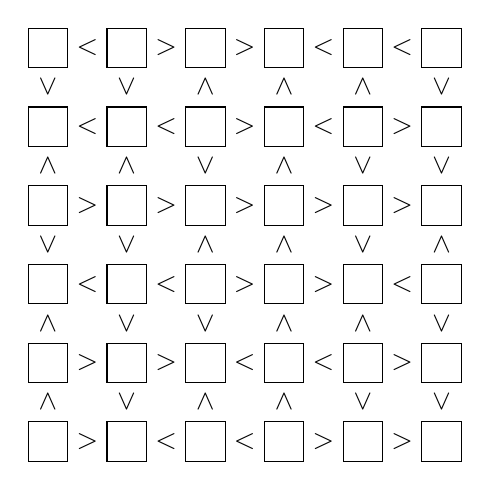
\begin{tikzpicture}[scale=0.5]

% ===== Vẽ các ô (rời nhau) =====
\foreach \x in {0,2,4,6,8,10} {
    \foreach \y in {0,2,4,6,8,10} {
        \draw (\x,\y) rectangle ++(1,1);
    }
}

% ===== Horizontal constraints =====
% Row 1
\node at (0.5+1,10.5) {$<$};
\node at (2.5+1,10.5) {$>$};
\node at (4.5+1,10.5) {$>$};
\node at (6.5+1,10.5) {$<$};
\node at (8.5+1,10.5) {$<$};

% Row 2
\node at (0.5+1,8.5) {$<$};
\node at (2.5+1,8.5) {$<$};
\node at (4.5+1,8.5) {$>$};
\node at (6.5+1,8.5) {$<$};
\node at (8.5+1,8.5) {$>$};

% Row 3
\node at (0.5+1,6.5) {$>$};
\node at (2.5+1,6.5) {$>$};
\node at (4.5+1,6.5) {$>$};
\node at (6.5+1,6.5) {$>$};
\node at (8.5+1,6.5) {$>$};

% Row 4
\node at (0.5+1,4.5) {$<$};
\node at (2.5+1,4.5) {$<$};
\node at (4.5+1,4.5) {$>$};
\node at (6.5+1,4.5) {$>$};
\node at (8.5+1,4.5) {$<$};

% Row 5
\node at (0.5+1,2.5) {$>$};
\node at (2.5+1,2.5) {$>$};
\node at (4.5+1,2.5) {$<$};
\node at (6.5+1,2.5) {$<$};
\node at (8.5+1,2.5) {$>$};

% Row 6
\node at (0.5+1,0.5) {$>$};
\node at (2.5+1,0.5) {$<$};
\node at (4.5+1,0.5) {$<$};
\node at (6.5+1,0.5) {$>$};
\node at (8.5+1,0.5) {$>$};

% ===== Vertical constraints =====
% Between row 1 & 2
\node at (0.5,9.5) {$\vee$};
\node at (2.5,9.5) {$\vee$};
\node at (4.5,9.5) {$\wedge$};
\node at (6.5,9.5) {$\wedge$};
\node at (8.5,9.5) {$\wedge$};
\node at (10.5,9.5) {$\vee$};

% Row 2 & 3
\node at (0.5,7.5) {$\wedge$};
\node at (2.5,7.5) {$\wedge$};
\node at (4.5,7.5) {$\vee$};
\node at (6.5,7.5) {$\wedge$};
\node at (8.5,7.5) {$\vee$};
\node at (10.5,7.5) {$\vee$};

% Row 3 & 4
\node at (0.5,5.5) {$\vee$};
\node at (2.5,5.5) {$\vee$};
\node at (4.5,5.5) {$\wedge$};
\node at (6.5,5.5) {$\wedge$};
\node at (8.5,5.5) {$\vee$};
\node at (10.5,5.5) {$\wedge$};

% Row 4 & 5
\node at (0.5,3.5) {$\wedge$};
\node at (2.5,3.5) {$\vee$};
\node at (4.5,3.5) {$\vee$};
\node at (6.5,3.5) {$\wedge$};
\node at (8.5,3.5) {$\wedge$};
\node at (10.5,3.5) {$\vee$};

% Row 5 & 6
\node at (0.5,1.5) {$\wedge$};
\node at (2.5,1.5) {$\vee$};
\node at (4.5,1.5) {$\wedge$};
\node at (6.5,1.5) {$\wedge$};
\node at (8.5,1.5) {$\vee$};
\node at (10.5,1.5) {$\vee$};

\end{tikzpicture}
\end{center}

\textbf{Kết quả:}
\begin{table}[H]
\centering
\begin{tabular}{|l|l|c|c|c|c|c|}
\hline
\textbf{Input} & \textbf{Method} & \textbf{Runtime (s)} & \textbf{Memory (MB)} & \textbf{Nodes} & \textbf{Solved} & \textbf{Timeout} \\
\hline
input\_05.txt & Forward Chaining & 24.12 & 24.92 & 914 & True & False \\
input\_05.txt & A* (Heuristic 1) & 3.81 & 17.36 & 5,177 & True & False \\
input\_05.txt & A* (Heuristic 2) & 0.25 & 0.62 & 37 & True & False \\
input\_05.txt & Brute Force & 300.00 & 0.15 & 3,042,329 & False & True \\
input\_05.txt & Backtracking & 0.17 & 14.66 & 3,693 & True & False \\
\hline
\end{tabular}
\caption{Kết quả benchmark cho input\_05.txt}
\end{table}

\paragraph{So sánh và đánh giá:}

\begin{itemize}
\item \textbf{Forward Chaining:}
\begin{itemize}
    \item Thời gian chạy 24.12s, bộ nhớ 24.92MB, mở rộng 914 nodes.
    \item Tìm được nghiệm thành công.
    \item Chi phí suy luận tăng lên đáng kể khi bài toán phức tạp hơn. Tuy nhiên, vẫn tìm được nghiệm nhờ constraint propagation, cho thấy lợi ích của phương pháp này cho bài toán không có clue.
\end{itemize}

\item \textbf{A* với Heuristic 1:}
\begin{itemize}
    \item Thời gian chạy 3.81s, bộ nhớ 17.36MB, mở rộng 5,177 nodes.
    \item Tìm được nghiệm thành công.
    \item Heuristic 1 nhanh hơn Forward Chaining gấp 6 lần, nhưng mở rộng nhiều node hơn (5,177 vs 914), cho thấy heuristic này vẫn chưa đủ mạnh cho bài toán phức tạp.
\end{itemize}

\item \textbf{A* với Heuristic 2:}
\begin{itemize}
    \item Thời gian chạy 0.25s, bộ nhớ tối thiểu (0.62MB), mở rộng 37 nodes.
    \item Tìm được nghiệm thành công.
    \item A* Heuristic 2 nhanh gấp 96 lần so với Forward Chaining, gấp 15 lần so với Heuristic 1. Mở rộng chỉ 37 nodes cho thấy heuristic này rất chính xác.
    \item Điều đặc biệt là số node mở rộng bằng với Input-04, cho thấy heuristic 2 tìm được đường dẫn tối ưu ngay lập tức.
\end{itemize}

\item \textbf{Brute Force:}
\begin{itemize}
    \item Timeout sau 300s, mở rộng 3,042,329 nodes.
    \item Không tìm được nghiệm.
    \item Brute Force hoàn toàn không khả thi cho bài toán 6x6 với constraints dày đặc. Chi phí tìm kiếm không có cắt tỉa là cực lớn.
\end{itemize}

\item \textbf{Backtracking:}
\begin{itemize}
    \item Thời gian chạy 0.17s, bộ nhớ 14.66MB, mở rộng 3,693 nodes.
    \item Tìm được nghiệm thành công.
    \item Backtracking tuy không nhanh bằng A* Heuristic 2 (0.17s vs 0.25s), nhưng vẫn hoàn toàn vượt trội so với Brute Force. Hiệu suất ổn định cho phép xử lý các bài toán phức tạp hơn.
\end{itemize}

\end{itemize}

\textbf{So sánh tổng thể:}

\begin{itemize}
    \item Về \textbf{khả năng xử lý bài toán phức tạp}:
    \begin{itemize}
        \item A* Heuristic 2 là phương pháp duy nhất cho performance xuất sắc (0.25s).
        \item Backtracking và A* Heuristic 1 vẫn xử lý được nhưng chậm hơn.
        \item Forward Chaining chậm đáng kể nhưng vẫn khả thi (24.12s).
        \item Brute Force hoàn toàn bất lực (timeout).
    \end{itemize}
    
    \item Về \textbf{khả năng mở rộng của heuristic}:
    \begin{itemize}
        \item Heuristic 2 mở rộng ổn định (37 nodes, bằng Input-04) cho thấy tính ổn định tuyệt vời khi kích thước bài toán tăng.
        \item Heuristic 1 mở rộng tăng theo kích thước bài toán (5,177 nodes), cho thấy hiệu quả giảm sút khi bài toán phức tạp hơn.
    \end{itemize}
    
    \item Về \textbf{vai trò của cắt tỉa}:
    \begin{itemize}
        \item Sự khác biệt giữa Brute Force (timeout) và Backtracking (0.17s) cho thấy cắt tỉa là thiết yếu cho bài toán phức tạp.
        \item Cắt tỉa giảm không gian tìm kiếm từ hơn 3 triệu nodes xuống chỉ 3,693 nodes.
    \end{itemize}
    
    \item Về \textbf{vai trò của heuristic}:
    \begin{itemize}
        \item Heuristic 2 giảm không gian tìm kiếm từ 3,693 nodes (Backtracking) xuống còn 37 nodes (A* Heuristic 2).
        \item Heuristic tốt là chìa khóa để đạt performance xuất sắc trên bài toán phức tạp.
    \end{itemize}
    
    \item Về \textbf{tác dụng của constraint propagation}:
    \begin{itemize}
        \item Forward Chaining với constraint propagation giúp giảm nodes (914 nodes) so với Brute Force (3,042,329 nodes), cho thấy ứu thế của constraint propagation.
        \item Tuy nhiên, chi phí suy luận là lớn khi bài toán phức tạp.
    \end{itemize}
\end{itemize}

\section{Input-06}
\textbf{Mô tả testcase:}
Testcase Futoshiki kích thước $7 \times 7$ với độ khó cao. Số lượng ô được điền ban đầu (clues) rất ít, dẫn đến không gian tìm kiếm lớn.

Các ràng buộc (constraints) tồn tại ở cả chiều ngang và dọc nhưng có mật độ trung bình và phân bố không đồng đều, làm giảm hiệu quả cắt tỉa.

Đặc biệt, testcase này được thiết kế \textbf{không có nghiệm hợp lệ}, nhằm đánh giá khả năng của các thuật toán trong việc phát hiện bài toán vô nghiệm (unsatisfiable problem).

Do đó, bài toán không chỉ yêu cầu chiến lược tìm kiếm hiệu quả mà còn cần cơ chế phát hiện mâu thuẫn sớm để tránh bùng nổ không gian trạng thái.

\begin{center}
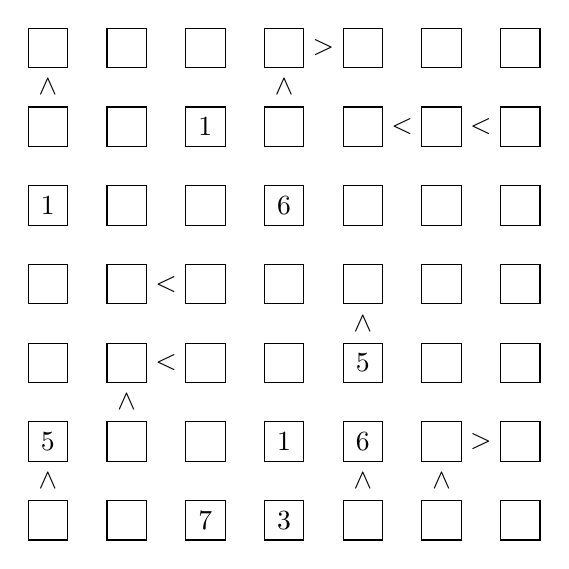
\begin{tikzpicture}[scale=0.5]

% ===== Vẽ các ô (rời nhau) =====
\foreach \x in {0,2,4,6,8,10,12} {
    \foreach \y in {0,2,4,6,8,10,12} {
        \draw (\x,\y) rectangle ++(1,1);
    }
}

% ===== Điền số =====
\node at (4.5,10.5) {1};

\node at (0.5,8.5) {1};
\node at (6.5,8.5) {6};

\node at (8.5,4.5) {5};

\node at (0.5,2.5) {5};
\node at (6.5,2.5) {1};
\node at (8.5,2.5) {6};

\node at (4.5,0.5) {7};
\node at (6.5,0.5) {3};

% ===== Horizontal constraints =====
\node at (6.5+1,12.5) {$>$};

\node at (8.5+1,10.5) {$<$};
\node at (10.5+1,10.5) {$<$};

\node at (2.5+1,6.5) {$<$};

\node at (2.5+1,4.5) {$<$};

\node at (10.5+1,2.5) {$>$};

% ===== Vertical constraints =====
\node at (0.5,11.5) {$\wedge$};
\node at (6.5,11.5) {$\wedge$};

\node at (8.5,5.5) {$\wedge$};

\node at (2.5,3.5) {$\wedge$};

\node at (0.5,1.5) {$\wedge$};
\node at (8.5,1.5) {$\wedge$};
\node at (10.5,1.5) {$\wedge$};

\end{tikzpicture}
\end{center}

\textbf{Kết quả:}
\begin{table}[H]
\centering
\begin{tabular}{|l|l|c|c|c|c|c|}
\hline
\textbf{Input} & \textbf{Method} & \textbf{Runtime (s)} & \textbf{Memory (MB)} & \textbf{Nodes} & \textbf{Solved} & \textbf{Timeout} \\
\hline
input\_06.txt & Forward Chaining & 0.09 & 3.05 & 1 & False & False \\
input\_06.txt & A* (Heuristic 1) & 300.00 & 1905.46 & 182,217 & False & True \\
input\_06.txt & A* (Heuristic 2) & 300.00 & 325.93 & 80,879 & False & True \\
input\_06.txt & Brute Force & 300.00 & 0.15 & 2,428,877 & False & True \\
input\_06.txt & Backtracking & 314.86 & 10589.39 & 2,237,011 & False & True \\
\hline
\end{tabular}
\caption{Kết quả benchmark cho input\_06.txt}
\end{table}

\paragraph{So sánh và đánh giá:}

\begin{itemize}
\item \textbf{Forward Chaining:}
\begin{itemize}
    \item Thời gian chạy rất thấp (0.089s), bộ nhớ sử dụng nhỏ (3.05MB), và chỉ mở rộng 1 node.
    \item Không tìm được nghiệm.
    \item Đây là kết quả hợp lý vì bài toán không có nghiệm. Phương pháp suy luận tiến đã nhanh chóng phát hiện mâu thuẫn thông qua constraint propagation mà không cần tìm kiếm sâu.
    \item Điều này cho thấy Forward Chaining hiệu quả trong việc phát hiện sớm trạng thái vô nghiệm.
\end{itemize}

\item \textbf{A* với Heuristic 1:}
\begin{itemize}
    \item Bị timeout sau 300s, mở rộng 182,217 nodes và sử dụng bộ nhớ lớn (1905.46MB).
    \item Không phát hiện được bài toán vô nghiệm trong thời gian cho phép.
    \item Điều này cho thấy heuristic 1 không đủ mạnh để dẫn dắt tìm kiếm tới các vùng mâu thuẫn sớm, dẫn đến việc khám phá không gian trạng thái một cách kém hiệu quả.
\end{itemize}

\item \textbf{A* với Heuristic 2:}
\begin{itemize}
    \item Cũng bị timeout, nhưng số node mở rộng giảm đáng kể (80,879 nodes) và bộ nhớ thấp hơn (325.93MB).
    \item Hiệu quả hơn heuristic 1 trong việc thu hẹp không gian tìm kiếm.
    \item Tuy nhiên vẫn chưa đủ để phát hiện bài toán vô nghiệm trong giới hạn thời gian.
\end{itemize}

\item \textbf{Brute Force:}
\begin{itemize}
    \item Mở rộng số lượng node cực lớn (2,428,877 nodes) và bị timeout.
    \item Không thể kết luận vô nghiệm do phải duyệt gần như toàn bộ không gian trạng thái.
    \item Đây là hạn chế cố hữu của phương pháp không có cắt tỉa.
\end{itemize}

\item \textbf{Backtracking:}
\begin{itemize}
    \item Mở rộng hơn 2 triệu nodes và vượt quá thời gian giới hạn (314.86s).
    \item Có cải thiện so với brute force nhờ cắt tỉa, nhưng vẫn không đủ để kết luận vô nghiệm trong thời gian hợp lý.
    \item Bộ nhớ rất cao do chi phí lưu trạng thái và đệ quy.
\end{itemize}

\end{itemize}

\textbf{So sánh tổng thể:}

\begin{itemize}
    \item Về \textbf{khả năng phát hiện vô nghiệm}:
    \begin{itemize}
        \item Forward Chaining là phương pháp duy nhất phát hiện nhanh trạng thái vô nghiệm nhờ cơ chế suy luận ràng buộc.
        \item Các phương pháp còn lại không thể kết luận trong thời gian giới hạn.
    \end{itemize}
    
    \item Về \textbf{hiệu quả heuristic}:
    \begin{itemize}
        \item Heuristic 2 tốt hơn Heuristic 1 (ít node hơn, ít bộ nhớ hơn).
        \item Tuy nhiên cả hai đều chưa đủ mạnh để dẫn dắt tìm kiếm tới mâu thuẫn sớm.
    \end{itemize}
    
    \item Về \textbf{chi phí tìm kiếm}:
    \begin{itemize}
        \item Brute Force và Backtracking có chi phí rất lớn do phải duyệt gần như toàn bộ không gian trạng thái.
        \item A* giúp giảm đáng kể số node, nhưng vẫn không đủ để xử lý bài toán vô nghiệm hiệu quả.
    \end{itemize}
    
    \item Về \textbf{vai trò của suy luận ràng buộc}:
    \begin{itemize}
        \item Forward Chaining cho thấy ưu thế rõ rệt trong việc phát hiện mâu thuẫn sớm.
        \item Điều này nhấn mạnh tầm quan trọng của constraint propagation trong các bài toán CSP vô nghiệm.
    \end{itemize}
\end{itemize}

\section{Input-07}
\textbf{Mô tả testcase:}

Testcase Futoshiki kích thước $7 \times 7$ không chứa bất kỳ giá trị khởi tạo (clue) hay ràng buộc bất đẳng thức (constraint) nào. Do đó, toàn bộ lưới ban đầu hoàn toàn trống và không có thông tin định hướng lời giải.

Trong trường hợp này, bài toán có không gian nghiệm rất lớn với nhiều nghiệm hợp lệ, do không bị giới hạn bởi các điều kiện ràng buộc. Việc thiếu constraint khiến các kỹ thuật suy luận không phát huy hiệu quả, trong khi các thuật toán tìm kiếm có thể nhanh chóng tìm được một nghiệm bất kỳ.

Testcase này chủ yếu dùng để đánh giá khả năng tìm nghiệm đầu tiên và hiệu năng cơ bản của các thuật toán trong môi trường không có thông tin định hướng.

\begin{center}

\begin{tikzpicture}[scale=0.5]

% ===== Vẽ các ô (rời nhau) =====
\foreach \x in {0,2,4,6,8,10,12} {
    \foreach \y in {0,2,4,6,8,10,12} {
        \draw (\x,\y) rectangle ++(1,1);
    }
}

% ===== Không có số =====

% ===== Không có ràng buộc ngang =====

% ===== Không có ràng buộc dọc =====

\end{tikzpicture}
\end{center}

\textbf{Kết quả:}
\begin{table}[H]
\centering
\begin{tabular}{|l|l|c|c|c|c|c|}
\hline
\textbf{Input} & \textbf{Method} & \textbf{Runtime (s)} & \textbf{Memory (MB)} & \textbf{Nodes} & \textbf{Solved} & \textbf{Timeout} \\
\hline
input\_07.txt & Forward Chaining & 0.62 & 36.87 & 26 & True & False \\
input\_07.txt & A* (Heuristic 1) & 300.00 & 2768.83 & 73,799 & False & True \\
input\_07.txt & A* (Heuristic 2) & 1.28 & 1.51 & 102 & True & False \\
input\_07.txt & Brute Force & 0.01 & 0.01 & 132 & True & False \\
input\_07.txt & Backtracking & 0.00 & 0.39 & 132 & True & False \\
\hline
\end{tabular}
\caption{Kết quả benchmark cho input\_07.txt}
\end{table}

\paragraph{So sánh và đánh giá:}

\begin{itemize}

\item \textbf{Forward Chaining:}
\begin{itemize}
    \item Thời gian chạy thấp (0.62s), số node mở rộng rất ít (26 nodes).
    \item Tìm được nghiệm thành công.
    \item Mặc dù không có nhiều ràng buộc để suy luận, phương pháp vẫn hoạt động hiệu quả do bài toán không yêu cầu tìm kiếm sâu.
\end{itemize}

\item \textbf{A* với Heuristic 1:}
\begin{itemize}
    \item Bị timeout sau 300s, mở rộng 73,799 nodes và tiêu tốn bộ nhớ lớn (2768.83MB).
    \item Hiệu năng kém do heuristic không cung cấp thông tin hữu ích trong trường hợp không có ràng buộc, dẫn đến việc tìm kiếm gần như mù.
\end{itemize}

\item \textbf{A* với Heuristic 2:}
\begin{itemize}
    \item Giải được bài toán trong thời gian ngắn (1.28s), mở rộng 102 nodes và sử dụng bộ nhớ rất thấp (1.51MB).
    \item Hoạt động tốt hơn Heuristic 1 nhờ khả năng định hướng tìm kiếm hợp lý hơn, dù bài toán không có nhiều thông tin ràng buộc.
\end{itemize}

\item \textbf{Brute Force:}
\begin{itemize}
    \item Giải rất nhanh (0.01s) với 132 nodes.
    \item Do bài toán có nhiều nghiệm, brute force dễ dàng tìm được một nghiệm mà không cần khám phá toàn bộ không gian.
\end{itemize}

\item \textbf{Backtracking:}
\begin{itemize}
    \item Là phương pháp nhanh nhất (0.0045s), với 132 nodes.
    \item Hiệu quả cao nhờ dừng sớm khi tìm được nghiệm đầu tiên.
\end{itemize}

\end{itemize}

\textbf{So sánh tổng thể:}

\begin{itemize}
    \item Về \textbf{khả năng giải bài}: hầu hết các phương pháp (trừ A* Heuristic 1) đều giải được nhanh chóng.
    
    \item Về \textbf{hiệu quả heuristic}:
    \begin{itemize}
        \item Heuristic 2 vượt trội so với Heuristic 1.
        \item Heuristic 1 không phù hợp trong trường hợp thiếu ràng buộc.
    \end{itemize}
    
    \item Về \textbf{chi phí tìm kiếm}:
    \begin{itemize}
        \item Brute Force và Backtracking có chi phí rất thấp do dừng sớm.
        \item A* (H1) có chi phí rất cao do mở rộng nhiều node không cần thiết.
    \end{itemize}
    
    \item Về \textbf{ảnh hưởng của ràng buộc}:
    \begin{itemize}
        \item Việc không có constraint khiến bài toán trở nên “dễ” theo nghĩa tìm nghiệm đầu tiên.
        \item Tuy nhiên, heuristic trở nên kém hiệu quả do thiếu thông tin định hướng.
    \end{itemize}

\end{itemize}

\section{Input-08}
\paragraph{Mô tả testcase:}

Testcase Futoshiki kích thước $7 \times 7$ với số lượng ô được điền ban đầu (clue) ít và phân bố rải rác trên lưới. 

Hệ thống ràng buộc (constraints) tồn tại ở cả chiều ngang và dọc với mật độ trung bình và phân bố không đồng đều, tạo ra một số vùng có khả năng suy luận tốt trong khi các vùng khác gần như không có thông tin định hướng.

Sự kết hợp này dẫn đến không gian tìm kiếm lớn nhưng vẫn có khả năng cắt tỉa cục bộ, khiến bài toán có độ khó cao và phù hợp để đánh giá hiệu quả của heuristic trong việc định hướng tìm kiếm.
\begin{center}
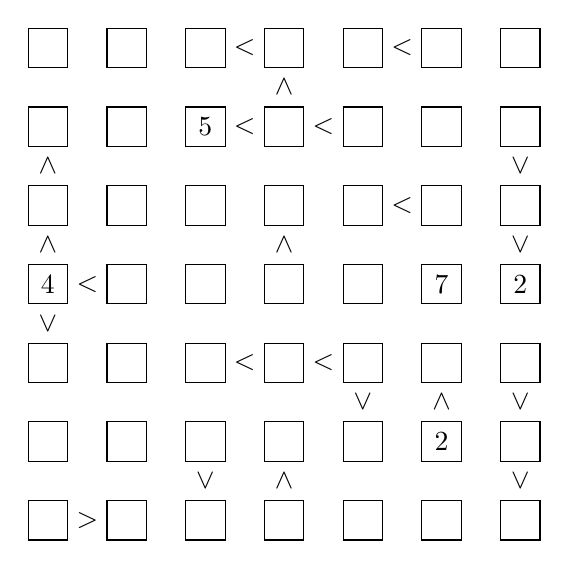
\begin{tikzpicture}[scale=0.5]

% ===== Vẽ các ô (rời nhau) =====
\foreach \x in {0,2,4,6,8,10,12} {
    \foreach \y in {0,2,4,6,8,10,12} {
        \draw (\x,\y) rectangle ++(1,1);
    }
}

% ===== Điền số =====
\node at (4.5,10.5) {5};

\node at (0.5,6.5) {4};
\node at (10.5,6.5) {7};
\node at (12.5,6.5) {2};

\node at (10.5,2.5) {2};

% ===== Dấu < (horizontal) =====
\node at (5.5,12.5) {$<$};
\node at (9.5,12.5) {$<$};

\node at (5.5,10.5) {$<$};
\node at (7.5,10.5) {$<$};

\node at (9.5,8.5) {$<$};

\node at (1.5,6.5) {$<$};

\node at (5.5,4.5) {$<$};
\node at (7.5,4.5) {$<$};

\node at (1.5,0.5) {$>$};

% ===== Dấu ^ (vertical) =====
\node at (6.5,11.5) {$\wedge$};

\node at (0.5,9.5) {$\wedge$};
\node at (12.5,9.5) {$\vee$};

\node at (0.5,7.5) {$\wedge$};
\node at (6.5,7.5) {$\wedge$};
\node at (12.5,7.5) {$\vee$};

\node at (0.5,5.5) {$\vee$};

\node at (8.5,3.5) {$\vee$};
\node at (10.5,3.5) {$\wedge$};
\node at (12.5,3.5) {$\vee$};

\node at (4.5,1.5) {$\vee$};
\node at (6.5,1.5) {$\wedge$};
\node at (12.5,1.5) {$\vee$};

\end{tikzpicture}
\end{center}

\paragraph{Kết quả:}
\begin{table}[H]
\centering
\begin{tabular}{|l|l|c|c|c|c|c|}
\hline
\textbf{Input} & \textbf{Method} & \textbf{Runtime (s)} & \textbf{Memory (MB)} & \textbf{Nodes} & \textbf{Solved} & \textbf{Timeout} \\
\hline
input\_08.txt & Forward Chaining & 35.35 & 37.11 & 1,090 & True & False \\
input\_08.txt & A* (Heuristic 1) & 300.00 & 1747.70 & 271,563 & False & True \\
input\_08.txt & A* (Heuristic 2) & 5.71 & 2.60 & 132 & True & False \\
input\_08.txt & Brute Force & 300.00 & 0.15 & 2,253,684 & False & True \\
input\_08.txt & Backtracking & 5.11 & 479.79 & 101,260 & True & False \\
\hline
\end{tabular}
\caption{Kết quả benchmark cho input\_08.txt}
\end{table}

\paragraph{So sánh và đánh giá:}
\begin{itemize}
\item \textbf{Forward Chaining:}
\begin{itemize}
    \item Giải được bài toán trong 35.35s với 1,090 nodes.
    \item Bộ nhớ sử dụng ở mức trung bình (37.11MB).
    \item Cho thấy suy luận ràng buộc có hiệu quả nhất định trong việc giảm không gian tìm kiếm, nhưng vẫn cần thời gian đáng kể để hội tụ.
\end{itemize}

\item \textbf{A* với Heuristic 1:}
\begin{itemize}
    \item Bị timeout sau 300s, mở rộng 271,563 nodes và tiêu tốn bộ nhớ lớn (1747.7MB).
    \item Heuristic 1 không đủ mạnh để định hướng tìm kiếm hiệu quả, dẫn đến việc khám phá nhiều trạng thái không cần thiết.
\end{itemize}

\item \textbf{A* với Heuristic 2:}
\begin{itemize}
    \item Giải thành công trong thời gian ngắn (5.71s), chỉ mở rộng 132 nodes.
    \item Bộ nhớ sử dụng rất thấp (2.6MB).
    \item Đây là phương pháp hiệu quả nhất trong testcase này, cho thấy heuristic 2 có khả năng định hướng tìm kiếm rất tốt.
\end{itemize}

\item \textbf{Brute Force:}
\begin{itemize}
    \item Bị timeout với số node mở rộng rất lớn (2,253,684 nodes).
    \item Không có cơ chế cắt tỉa nên không phù hợp với bài toán có không gian tìm kiếm lớn.
\end{itemize}

\item \textbf{Backtracking:}
\begin{itemize}
    \item Giải được bài toán trong 5.11s, nhưng mở rộng tới 101,260 nodes.
    \item Bộ nhớ khá cao (479.79MB).
    \item Mặc dù có cắt tỉa, nhưng vẫn kém hiệu quả hơn A* với heuristic tốt.
\end{itemize}

\end{itemize}

\textbf{So sánh tổng thể:}

\begin{itemize}
    \item Về \textbf{khả năng giải bài}:
    \begin{itemize}
        \item Forward Chaining, A* (Heuristic 2) và Backtracking đều giải được bài toán.
        \item A* (Heuristic 1) và Brute Force thất bại do timeout.
    \end{itemize}
    
    \item Về \textbf{hiệu quả heuristic}:
    \begin{itemize}
        \item Heuristic 2 vượt trội so với Heuristic 1 cả về thời gian, bộ nhớ và số node mở rộng.
        \item Điều này cho thấy tầm quan trọng của việc thiết kế heuristic phù hợp.
    \end{itemize}
    
    \item Về \textbf{chi phí tìm kiếm}:
    \begin{itemize}
        \item A* (Heuristic 2) có chi phí thấp nhất (132 nodes).
        \item Backtracking tốn nhiều node hơn nhưng vẫn trong giới hạn chấp nhận được.
        \item Brute Force là kém nhất do không có cắt tỉa.
    \end{itemize}
    
    \item Về \textbf{vai trò của ràng buộc}:
    \begin{itemize}
        \item Các constraint giúp giảm đáng kể không gian tìm kiếm, cho phép các thuật toán như A* (H2) hoạt động hiệu quả.
    \end{itemize}

\end{itemize}

\section{Input-09}
\textbf{Mô tả testcase:}
\textbf{Mô tả testcase:}

Testcase Futoshiki kích thước $9 \times 9$ với số lượng clue ít và phân bố không đồng đều trên lưới. 

Hệ thống ràng buộc (constraints) tương đối dày và xuất hiện ở cả chiều ngang và dọc, tuy nhiên vẫn tồn tại nhiều vùng thiếu thông tin định hướng.

Sự kết hợp giữa kích thước lớn, số lượng clue hạn chế và constraint chưa đủ mạnh để ràng buộc toàn cục khiến không gian tìm kiếm rất lớn, làm tăng đáng kể độ khó của bài toán.
\begin{center}
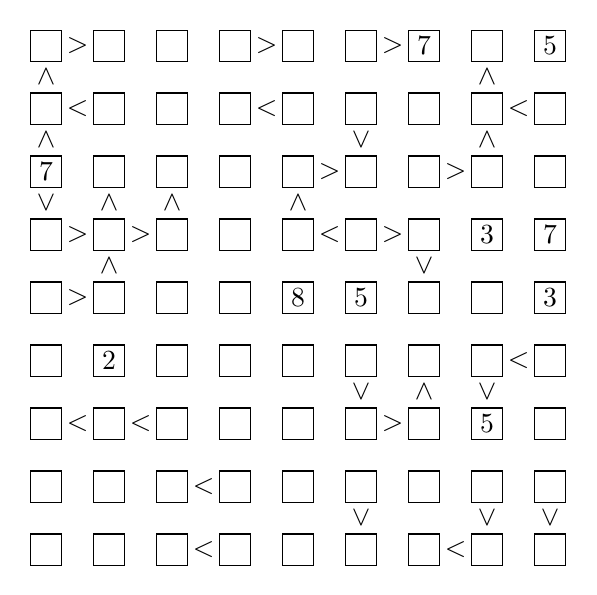
\begin{tikzpicture}[scale=0.4]

% ===== Vẽ các ô (rời nhau) =====
\foreach \x in {0,2,4,6,8,10,12,14,16} {
    \foreach \y in {0,2,4,6,8,10,12,14,16} {
        \draw (\x,\y) rectangle ++(1,1);
    }
}

% ===== Điền số =====
\node at (12.5,16.5) {7};
\node at (16.5,16.5) {5};

\node at (0.5,12.5) {7};

\node at (14.5,10.5) {3};
\node at (16.5,10.5) {7};

\node at (8.5,8.5) {8};
\node at (10.5,8.5) {5};
\node at (16.5,8.5) {3};

\node at (2.5,6.5) {2};

\node at (14.5,4.5) {5};

% ===== Horizontal constraints =====
\node at (0.5+1,16.5) {$>$};
\node at (6.5+1,16.5) {$>$};
\node at (10.5+1,16.5) {$>$};

\node at (0.5+1,14.5) {$<$};
\node at (6.5+1,14.5) {$<$};
\node at (14.5+1,14.5) {$<$};

\node at (8.5+1,12.5) {$>$};
\node at (12.5+1,12.5) {$>$};

\node at (0.5+1,10.5) {$>$};
\node at (2.5+1,10.5) {$>$};
\node at (8.5+1,10.5) {$<$};
\node at (10.5+1,10.5) {$>$};

\node at (0.5+1,8.5) {$>$};

\node at (14.5+1,6.5) {$<$};

\node at (0.5+1,4.5) {$<$};
\node at (2.5+1,4.5) {$<$};
\node at (10.5+1,4.5) {$>$};

\node at (4.5+1,2.5) {$<$};

\node at (4.5+1,0.5) {$<$};
\node at (12.5+1,0.5) {$<$};

% ===== Vertical constraints =====
\node at (0.5,15.5) {$\wedge$};
\node at (14.5,15.5) {$\wedge$};

\node at (0.5,13.5) {$\wedge$};
\node at (10.5,13.5) {$\vee$};
\node at (14.5,13.5) {$\wedge$};

\node at (0.5,11.5) {$\vee$};
\node at (2.5,11.5) {$\wedge$};
\node at (4.5,11.5) {$\wedge$};
\node at (8.5,11.5) {$\wedge$};

\node at (2.5,9.5) {$\wedge$};
\node at (12.5,9.5) {$\vee$};

\node at (10.5,5.5) {$\vee$};
\node at (12.5,5.5) {$\wedge$};
\node at (14.5,5.5) {$\vee$};

\node at (10.5,1.5) {$\vee$};
\node at (14.5,1.5) {$\vee$};
\node at (16.5,1.5) {$\vee$};

\end{tikzpicture}
\end{center}

\textbf{Kết quả:}
\begin{table}[H]
\centering
\begin{tabular}{|l|l|c|c|c|c|c|}
\hline
\textbf{Input} & \textbf{Method} & \textbf{Runtime (s)} & \textbf{Memory (MB)} & \textbf{Nodes} & \textbf{Solved} & \textbf{Timeout} \\
\hline
input\_09.txt & Forward Chaining & 300.15 & 194.51 & 3,145 & False & True \\
input\_09.txt & A* (Heuristic 1) & 300.00 & 2834.59 & 66,178 & False & True \\
input\_09.txt & A* (Heuristic 2) & 300.01 & 204.55 & 4,138 & False & True \\
input\_09.txt & Brute Force & 300.00 & 0.15 & 1,151,494 & False & True \\
input\_09.txt & Backtracking & 300.72 & 10602.58 & 1,722,995 & False & True \\
\hline
\end{tabular}
\caption{Kết quả benchmark cho input\_09.txt}
\end{table}

\textbf{So sánh và đánh giá:}
\begin{itemize}
\item \textbf{Forward Chaining:}
\begin{itemize}
    \item Bị timeout sau 300s, chỉ mở rộng 3,145 nodes.
    \item Bộ nhớ sử dụng ở mức trung bình (194.51MB).
    \item Mặc dù số node mở rộng không lớn, phương pháp không thể hội tụ do thiếu cơ chế tìm kiếm sâu, chỉ dựa vào suy luận ràng buộc.
\end{itemize}

\item \textbf{A* với Heuristic 1:}
\begin{itemize}
    \item Bị timeout với 66,178 nodes và bộ nhớ rất cao (2834.59MB).
    \item Heuristic 1 không đủ mạnh để định hướng tìm kiếm trong không gian trạng thái lớn, dẫn đến việc mở rộng nhiều trạng thái không cần thiết.
\end{itemize}

\item \textbf{A* với Heuristic 2:}
\begin{itemize}
    \item Cũng bị timeout, nhưng chỉ mở rộng 4,138 nodes và sử dụng bộ nhớ thấp hơn (204.55MB).
    \item So với Heuristic 1, hiệu quả tốt hơn rõ rệt, cho thấy heuristic 2 có khả năng định hướng tốt hơn.
    \item Tuy nhiên, vẫn chưa đủ mạnh để giải bài toán trong thời gian giới hạn.
\end{itemize}

\item \textbf{Brute Force:}
\begin{itemize}
    \item Mở rộng hơn 1.15 triệu nodes và bị timeout.
    \item Bộ nhớ thấp (0.15MB) do không lưu trữ nhiều trạng thái.
    \item Đây là phương pháp kém hiệu quả nhất về thời gian do không có cơ chế cắt tỉa.
\end{itemize}

\item \textbf{Backtracking:}
\begin{itemize}
    \item Mở rộng hơn 1.7 triệu nodes và vượt thời gian giới hạn (300.72s).
    \item Bộ nhớ rất cao (10602.58MB), phản ánh chi phí lớn trong việc duy trì trạng thái và recursion.
    \item Có cải thiện so với brute force nhờ cắt tỉa, nhưng vẫn không đủ hiệu quả.
\end{itemize}

\end{itemize}

\textbf{So sánh tổng thể:}

\begin{itemize}
    \item Về \textbf{khả năng giải bài}: tất cả các phương pháp đều thất bại (timeout), cho thấy đây là testcase cực khó.
    
    \item Về \textbf{hiệu quả heuristic}:
    \begin{itemize}
        \item Heuristic 2 tốt hơn Heuristic 1 (ít node hơn, ít bộ nhớ hơn).
        \item Tuy nhiên, cả hai đều không đủ mạnh để giải bài toán.
    \end{itemize}
    
    \item Về \textbf{chi phí tìm kiếm}:
    \begin{itemize}
        \item Brute Force và Backtracking có chi phí cực lớn (hàng triệu node).
        \item A* giúp giảm đáng kể số node, đặc biệt với Heuristic 2.
    \end{itemize}
    
    \item Về \textbf{vai trò của ràng buộc}:
    \begin{itemize}
        \item Mặc dù có nhiều ràng buộc, chúng vẫn chưa đủ mạnh để thu hẹp không gian tìm kiếm một cách hiệu quả.
    \end{itemize}

\end{itemize}

\section{Input-10}
\textbf{Mô tả testcase:}

Testcase Futoshiki kích thước $9 \times 9$ với độ khó rất cao. Số lượng giá trị khởi tạo (clues) rất ít và phân bố rời rạc, làm tăng đáng kể không gian tìm kiếm.

Hệ thống ràng buộc bất đẳng thức xuất hiện dày đặc ở cả hai chiều ngang và dọc, với mức độ phân bố tương đối phức tạp và không đồng đều. Điều này tạo ra nhiều phụ thuộc cục bộ nhưng không đủ mạnh để dẫn dắt trực tiếp đến nghiệm.

Sự kết hợp giữa \textbf{ít clue} và \textbf{nhiều constraint phức tạp} khiến bài toán vừa có không gian trạng thái lớn, vừa khó cắt tỉa hiệu quả. Do đó, testcase này được đánh giá là \textbf{rất khó}, đòi hỏi heuristic mạnh và chiến lược tìm kiếm tối ưu.
\begin{center}
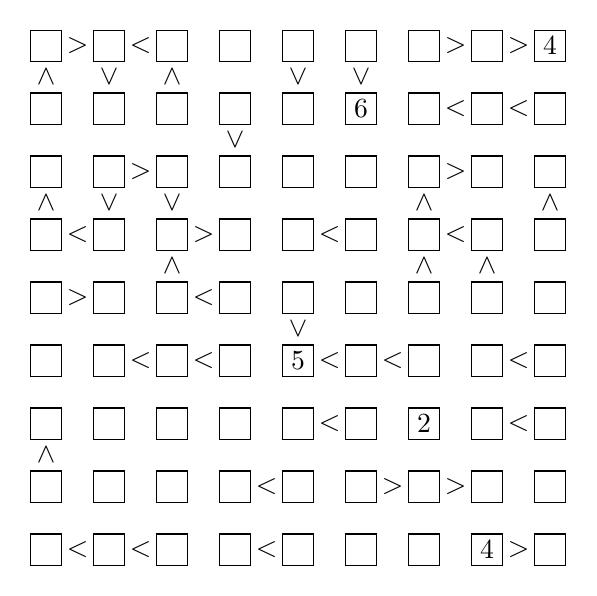
\begin{tikzpicture}[scale=0.4]

% ===== Vẽ các ô =====
\foreach \x in {0,2,4,6,8,10,12,14,16} {
    \foreach \y in {0,2,4,6,8,10,12,14,16} {
        \draw (\x,\y) rectangle ++(1,1);
    }
}

% ===== Điền số =====
\node at (16.5,16.5) {4};

\node at (10.5,14.5) {6};

\node at (8.5,6.5) {5};

\node at (12.5,4.5) {2};

\node at (14.5,0.5) {4};

% ===== Horizontal constraints =====
% Row 1
\node at (0.5+1,16.5) {$>$};
\node at (2.5+1,16.5) {$<$};
\node at (12.5+1,16.5) {$>$};
\node at (14.5+1,16.5) {$>$};

% Row 2
\node at (12.5+1,14.5) {$<$};
\node at (14.5+1,14.5) {$<$};

% Row 3
\node at (2.5+1,12.5) {$>$};
\node at (12.5+1,12.5) {$>$};

% Row 4
\node at (0.5+1,10.5) {$<$};
\node at (4.5+1,10.5) {$>$};
\node at (8.5+1,10.5) {$<$};
\node at (12.5+1,10.5) {$<$};

% Row 5
\node at (0.5+1,8.5) {$>$};
\node at (4.5+1,8.5) {$<$};

% Row 6
\node at (2.5+1,6.5) {$<$};
\node at (4.5+1,6.5) {$<$};
\node at (8.5+1,6.5) {$<$};
\node at (10.5+1,6.5) {$<$};
\node at (14.5+1,6.5) {$<$};

% Row 7
\node at (8.5+1,4.5) {$<$};
\node at (14.5+1,4.5) {$<$};

% Row 8
\node at (6.5+1,2.5) {$<$};
\node at (10.5+1,2.5) {$>$};
\node at (12.5+1,2.5) {$>$};

% Row 9
\node at (0.5+1,0.5) {$<$};
\node at (2.5+1,0.5) {$<$};
\node at (6.5+1,0.5) {$<$};
\node at (14.5+1,0.5) {$>$};

% ===== Vertical constraints =====
\node at (0.5,15.5) {$\wedge$};
\node at (2.5,15.5) {$\vee$};
\node at (4.5,15.5) {$\wedge$};
\node at (8.5,15.5) {$\vee$};
\node at (10.5,15.5) {$\vee$};

\node at (6.5,13.5) {$\vee$};

\node at (0.5,11.5) {$\wedge$};
\node at (2.5,11.5) {$\vee$};
\node at (4.5,11.5) {$\vee$};
\node at (12.5,11.5) {$\wedge$};
\node at (16.5,11.5) {$\wedge$};

\node at (4.5,9.5) {$\wedge$};
\node at (12.5,9.5) {$\wedge$};
\node at (14.5,9.5) {$\wedge$};

\node at (8.5,7.5) {$\vee$};

\node at (0.5,3.5) {$\wedge$};

\end{tikzpicture}
\end{center}

\textbf{Kết quả:}
\begin{table}[H]
\centering
\begin{tabular}{|l|l|c|c|c|c|c|}
\hline
\textbf{Input} & \textbf{Method} & \textbf{Runtime (s)} & \textbf{Memory (MB)} & \textbf{Nodes} & \textbf{Solved} & \textbf{Timeout} \\
\hline
input\_10.txt & Forward Chaining & 300.22 & 208.27 & 3,060 & False & True \\
input\_10.txt & A* (Heuristic 1) & 300.00 & 2668.90 & 76,518 & False & True \\
input\_10.txt & A* (Heuristic 2) & 300.01 & 213.28 & 4,959 & False & True \\
input\_10.txt & Brute Force & 300.00 & 0.15 & 1,156,082 & False & True \\
input\_10.txt & Backtracking & 310.14 & 10589.40 & 1,720,780 & False & True \\
\hline
\end{tabular}
\caption{Kết quả benchmark cho input\_10.txt}
\end{table}

\paragraph{So sánh và đánh giá:}
\begin{itemize}
\item \textbf{Forward Chaining:}
\begin{itemize}
    \item Bị timeout sau 300s, mở rộng 3,060 nodes với mức bộ nhớ trung bình (208.27MB).
    \item Không tìm được nghiệm.
    \item Mặc dù có khả năng suy luận ràng buộc, phương pháp này không đủ mạnh để phát hiện mâu thuẫn hoặc hội tụ đến nghiệm trong không gian tìm kiếm lớn.
\end{itemize}

\item \textbf{A* với Heuristic 1:}
\begin{itemize}
    \item Bị timeout, mở rộng 76,518 nodes và tiêu tốn bộ nhớ rất lớn (2668.90MB).
    \item Hiệu năng kém cho thấy heuristic 1 không cung cấp đủ thông tin để định hướng tìm kiếm hiệu quả, dẫn đến việc mở rộng nhiều trạng thái không cần thiết.
\end{itemize}

\item \textbf{A* với Heuristic 2:}
\begin{itemize}
    \item Cũng bị timeout, nhưng chỉ mở rộng 4,959 nodes và sử dụng bộ nhớ thấp hơn đáng kể (213.28MB).
    \item So với heuristic 1, hiệu quả tốt hơn rõ rệt trong việc giảm không gian tìm kiếm.
    \item Tuy nhiên vẫn chưa đủ mạnh để giải bài toán trong giới hạn thời gian.
\end{itemize}

\item \textbf{Brute Force:}
\begin{itemize}
    \item Mở rộng hơn 1.15 triệu nodes và bị timeout.
    \item Bộ nhớ thấp (0.15MB) nhưng thời gian rất lớn do không có cơ chế cắt tỉa.
    \item Không phù hợp với bài toán có không gian trạng thái lớn như testcase này.
\end{itemize}

\item \textbf{Backtracking:}
\begin{itemize}
    \item Mở rộng hơn 1.72 triệu nodes và vượt thời gian giới hạn (310.14s).
    \item Bộ nhớ rất cao (10589.40MB), phản ánh chi phí lớn trong việc lưu trạng thái và đệ quy.
    \item Có cải thiện so với brute force nhờ cắt tỉa, nhưng vẫn không đủ hiệu quả.
\end{itemize}

\end{itemize}

\textbf{So sánh tổng thể:}

\begin{itemize}
    \item Về \textbf{khả năng giải bài}: tất cả các phương pháp đều không tìm được nghiệm trong thời gian giới hạn, cho thấy đây là một testcase \textbf{rất khó} (có thể có không gian nghiệm cực lớn hoặc tiềm ẩn mâu thuẫn).

    \item Về \textbf{hiệu quả heuristic}:
    \begin{itemize}
        \item Heuristic 2 vượt trội so với Heuristic 1 (ít node hơn, ít bộ nhớ hơn).
        \item Tuy nhiên cả hai vẫn chưa đủ mạnh để dẫn dắt tìm kiếm đến nghiệm hoặc phát hiện mâu thuẫn sớm.
    \end{itemize}

    \item Về \textbf{chi phí tìm kiếm}:
    \begin{itemize}
        \item Brute Force và Backtracking có chi phí cực lớn (hàng triệu node), thể hiện rõ hiện tượng bùng nổ không gian trạng thái.
        \item A* giúp giảm đáng kể số node, đặc biệt với heuristic 2, nhưng vẫn chưa đủ để giải quyết bài toán.
    \end{itemize}

    \item Về \textbf{vai trò của ràng buộc}:
    \begin{itemize}
        \item Mặc dù có nhiều ràng buộc, chúng chưa đủ mạnh hoặc chưa được khai thác hiệu quả để cắt tỉa không gian tìm kiếm.
        \item Điều này cho thấy việc kết hợp heuristic mạnh với kỹ thuật suy luận ràng buộc sâu hơn là cần thiết.
    \end{itemize}

\end{itemize}
